% ROZDZIAŁ 16 — skończone miary ze znakiem i zespolone
\chapter[Miary ze znakiem i zespolone]{Miary ze znakiem, miary zespolone i wariacja całkowita}
\label{ch:miary-ze-znakiem}

\section{Od miar dodatnich do miar przyjmujących wartości ujemne}
Dotychczas miara $\mu$ przyjmowała wartości w $[0,\infty]$.
W zastosowaniach pojawiają się różnice miar, np.
$\nu(E)=\int_E f(x)\,\mathrm d\mu(x)$ dla rzeczywistej
funkcji $f\in L^1(\mu)$, oraz miary zespolone
powstające przez całkowanie funkcji zespolonych.
W tym rozdziale zaczynamy od \emph{skończonych wartości},
aby nie tworzyć niezdefiniowanego wyrażenia $+\infty-\infty$.
O miarach ze znakiem przyjmujących jedną z wartości
nieskończonych wspomnimy osobno na końcu rozdziału;
główne twierdzenia udowadniamy dla miar skończenie wartościowych.

\begin{definicja}[Skończona miara ze znakiem]
\label{def:signed-measure-16}
Niech $(X,\mathcal F)$ będzie przestrzenią mierzalną.
\emph{Skończoną (skończenie wartościową) miarą ze znakiem}
nazywamy funkcję $\nu:\mathcal F\to\mathbb R$, dla której
$\nu(\varnothing)=0$ oraz dla dowolnych parami rozłącznych
$(E_n)_{n\ge1}\subset\mathcal F$ zachodzi
$\nu(\bigcup_{n\ge1}E_n)=\sum_{n\ge1}\nu(E_n)$.
Szereg po prawej jest wówczas zbieżny i — jako że równość
obowiązuje przy dowolnej permutacji zbiorów — bezwzględnie
zbieżny. Nie żądamy monotoniczności $\nu$.
\end{definicja}

\begin{przyklad}[Różnica skończonych miar]
Jeżeli $\mu_1,\mu_2$ są dodatnimi miarami na $\mathcal F$
i $\mu_1(X),\mu_2(X)<\infty$, to $\nu=\mu_1-\mu_2$
jest skończoną miarą ze znakiem.
Jeżeli $f\in L^1(\mu;\mathbb R)$, to
$\nu_f(E)=\int_E f\,\mathrm d\mu(x)$ jest skończoną miarą ze znakiem.
Jej przeliczalna addytywność wynika z całkowania sumy
funkcji charakterystycznych rozłącznych zbiorów, osobno dla $f^+$ i $f^-$.
\end{przyklad}

\begin{uwaga}[Ciągłość z góry i z dołu]
Dla skończonej miary ze znakiem $\nu$, jeśli
$E_n\uparrow E$, to $\nu(E_n)\to\nu(E)$, natomiast
jeśli $E_n\downarrow E$, to $\nu(E_n)\to\nu(E)$.
Pierwszy fakt otrzymujemy, rozkładając $E$ na rozłączne
przyrosty $E_1,E_2\setminus E_1,\dots$; drugi wynika
z pierwszego dla dopełnień oraz skończonej addytywności.
W odróżnieniu od miar nieujemnych nie jest potrzebne
założenie $\nu(E_1)<\infty$, bo wszystkie wartości
$\nu$ są rzeczywiste.
\end{uwaga}

\section{Dlaczego skończona miara ze znakiem jest ograniczona?}
\begin{lemat}[Ograniczoność zakresu]
\label{lem:bounded-signed-16}
Jeśli $\nu:\mathcal F\to\mathbb R$ jest skończoną
miarą ze znakiem, to $M:=\sup_{E\in\mathcal F}|\nu(E)|<\infty$.
\end{lemat}
\begin{proof}
Przypuśćmy przeciwnie, że wartości $\nu$ są nieograniczone
na podzbiorach $X$. Powiemy, że zbiór $B\in\mathcal F$
jest \emph{nieograniczony}, jeżeli
$\sup\{|\nu(A)|:A\in\mathcal F,A\subseteq B\}=\infty$.
Mamy więc nieograniczony zbiór $B_1=X$.
Wybieramy $A\subseteq B_1$ z
$|\nu(A)|>|\nu(B_1)|+2$. Ponieważ
$\nu(B_1\setminus A)=\nu(B_1)-\nu(A)$,
oba rozłączne zbiory $A$ i $B_1\setminus A$ mają
wartość $\nu$ o module większym niż $2$.
Co najmniej jeden z nich jest nieograniczony: gdyby oba
były ograniczone, dla każdego $C\subseteq B_1$ mielibyśmy
$\nu(C)=\nu(C\cap A)+\nu(C\cap(B_1\setminus A))$,
co dawałoby ograniczoność na $B_1$.
Jako $B_2$ wybieramy część nieograniczoną, a drugą
nazywamy $D_1$. Wtedy $|\nu(D_1)|>2$.
Powtarzając konstrukcję w $B_2$, otrzymujemy kolejne
nieograniczone $B_n$ i parami rozłączne $D_n$
o $|\nu(D_n)|>2$. Jednak przeliczalna addytywność
wymaga zbieżności szeregu $\sum_n\nu(D_n)$,
a więc w szczególności $\nu(D_n)\to0$.
Otrzymaliśmy sprzeczność.
\end{proof}

\section{Rozkład Hahna}
\begin{definicja}[Zbiór dodatni i ujemny]
\label{def:positive-negative-16}
Niech $\nu$ będzie skończoną miarą ze znakiem.
Zbiór $P\in\mathcal F$ nazywamy $\nu$-\emph{dodatnim},
jeżeli $\nu(A)\ge0$ dla każdego mierzalnego $A\subseteq P$.
Zbiór $N\in\mathcal F$ nazywamy $\nu$-\emph{ujemnym},
jeżeli $\nu(A)\le0$ dla każdego mierzalnego $A\subseteq N$.
Nierówność dla samego $\nu(P)$, bez kwantyfikacji po
wszystkich podzbiorach, nie wystarcza.
\end{definicja}

\begin{twierdzenie}[Rozkład Hahna]
\label{thm:hahn-16}
Dla każdej skończonej miary ze znakiem $\nu$ na
$(X,\mathcal F)$ istnieją rozłączne mierzalne zbiory
$P,N\in\mathcal F$ takie, że $X=P\cup N$,
$P$ jest $\nu$-dodatni, a $N$ jest $\nu$-ujemny.
Ponadto jeśli $(P',N')$ jest drugim takim rozkładem,
to $P\mathbin\triangle P'$ jest $\nu$-zerowy
w silnym sensie: $\nu(A)=0$ dla każdego mierzalnego
$A\subseteq P\mathbin\triangle P'$.
\end{twierdzenie}
\begin{proof}
\emph{Istnienie.} Na mocy lematu~\ref{lem:bounded-signed-16}
liczba $\alpha:=\sup\{\nu(A):A\in\mathcal F\}$ jest
skończona i $\alpha\ge0$. Dla $n\ge1$ wybieramy
$A_n\in\mathcal F$ z $\nu(A_n)>\alpha-2^{-n}$.
Dla każdego mierzalnego $B\subseteq A_n$ zachodzi
$\nu(B)\ge-2^{-n}$: w przeciwnym przypadku
$\nu(A_n\setminus B)=\nu(A_n)-\nu(B)>\alpha$,
sprzecznie z definicją $\alpha$.

Niech $F_m=\bigcup_{n\ge m}A_n$. Dla $k\ge m$,
przy dokładaniu $A_{k+1}$ do $\bigcup_{n=m}^kA_n$
dokładamy zbiór mierzalny zawarty w $A_{k+1}$,
a więc jego wartość $\nu$ jest nie mniejsza
niż $-2^{-(k+1)}$. Zatem
\[
\nu\left(\bigcup_{n=m}^kA_n\right)
\ge\nu(A_m)-\sum_{n=m+1}^k2^{-n}
>\alpha-2^{1-m}.
\]
Dla $k\to\infty$ ciągłość $\nu$ z dołu daje
$\nu(F_m)\ge\alpha-2^{1-m}$; z definicji
$\alpha$ mamy również $\nu(F_m)\le\alpha$.
Zbiory $F_m$ maleją, więc dla
$P:=\bigcap_{m\ge1}F_m$ ciągłość $\nu$ z góry daje
$\nu(P)=\lim_m\nu(F_m)=\alpha$.

Jeśli $B\subseteq P$ jest mierzalny, to
$\nu(P\setminus B)\le\alpha$ i
$\nu(B)=\nu(P)-\nu(P\setminus B)\ge0$.
Zatem $P$ jest dodatni. Jeżeli $B\subseteq N:=X\setminus P$,
to $\nu(P\cup B)=\alpha+\nu(B)\le\alpha$,
więc $\nu(B)\le0$. To dowodzi, że $N$ jest ujemny.

\emph{Jednoznaczność.} Zbiór $P\cap N'$ jest jednocześnie
podzbiorem zbioru dodatniego i ujemnego. Każdy jego
mierzalny podzbiór ma zatem miarę ze znakiem równą zero.
To samo dotyczy $N\cap P'$. Ich suma
$(P\cap N')\cup(N\cap P')=P\mathbin\triangle P'$ ma
więc wskazaną własność.
\end{proof}

\begin{przyklad}[Rozkład Hahna nie zależy tylko od znaku całkowitej masy]
Na $X=[0,1]$ z miarą Lebesgue'a połóżmy
$\nu(E)=\int_E(2x-1)\,\mathrm d\lambda_1(x)$.
Wtedy $P=[1/2,1]$ oraz $N=[0,1/2)$ tworzą rozkład
Hahna, chociaż $\nu(X)=0$. Dowolny fragment
zbioru $\{1/2\}$ można przenieść z $P$ do $N$;
nie zmienia to wartości $\nu$ na żadnym podzbiorze.
\end{przyklad}

\begin{center}
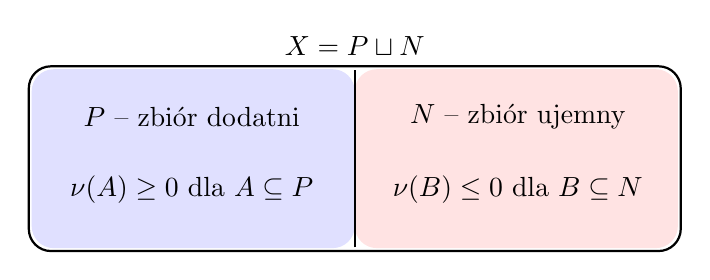
\begin{tikzpicture}[scale=0.92]
\draw[rounded corners=8pt,thick] (0,0) rectangle (9,2.55);
\fill[blue!12,rounded corners=8pt] (0.04,0.04) rectangle (4.5,2.51);
\fill[red!11,rounded corners=8pt] (4.5,0.04) rectangle (8.96,2.51);
\draw[thick] (4.5,0.05)--(4.5,2.5);
\node at (2.25,1.85) {$P$ -- zbiór dodatni};
\node at (6.75,1.85) {$N$ -- zbiór ujemny};
\node at (2.25,0.85) {$\nu(A)\ge0$ dla $A\subseteq P$};
\node at (6.75,0.85) {$\nu(B)\le0$ dla $B\subseteq N$};
\node[above] at (4.5,2.56) {$X=P\sqcup N$};
\end{tikzpicture}
\end{center}
\noindent Rysunek ilustruje kwantyfikację po \emph{wszystkich}
zbiorach mierzalnych zawartych w częściach $P$ i $N$;
nie wystarcza sam znak $\nu(P)$ oraz $\nu(N)$.

\section{Rozkład Jordana i wariacja całkowita}
\begin{definicja}[Wzajemna osobliwość]
\label{def:singular-16}
Dwie nieujemne miary $\mu_1,\mu_2$ na
$(X,\mathcal F)$ są \emph{wzajemnie osobliwe}, co zapisujemy
$\mu_1\perp\mu_2$, jeżeli istnieje $P\in\mathcal F$
taki, że $\mu_1(X\setminus P)=0$ oraz $\mu_2(P)=0$.
\end{definicja}

\begin{twierdzenie}[Rozkład Jordana]
\label{thm:jordan-16}
Niech $\nu$ będzie skończoną miarą ze znakiem.
Istnieje dokładnie jedna para skończonych miar nieujemnych
$(\nu^+,\nu^-)$ taka, że
$\nu=\nu^+-\nu^-$ i $\nu^+\perp\nu^-$.
Jeżeli $(P,N)$ jest rozkładem Hahna, to
\[
\nu^+(E)=\nu(E\cap P),\qquad
\nu^-(E)=-\nu(E\cap N)\quad(E\in\mathcal F).
\]
Ponadto $\nu^+(X)=\sup_E\nu(E)$ i
$\nu^-(X)=-\inf_E\nu(E)$.
\end{twierdzenie}
\begin{proof}
Dla rozkładu Hahna $P,N$ podane funkcje
są nieujemne i przeliczalnie addytywne, bo ich
argumenty $E\cap P$ i $E\cap N$ zachowują rozłączność.
Mamy $\nu(E)=\nu(E\cap P)+\nu(E\cap N)
=\nu^+(E)-\nu^-(E)$ oraz
$\nu^+(N)=\nu^-(P)=0$. Obie miary są skończone,
bo $\nu$ przyjmuje wartości rzeczywiste.

Jeżeli $\nu=\alpha-\beta$, gdzie $\alpha,\beta$ są
nieujemnymi miarami skończonymi i $\alpha\perp\beta$,
to istnieje $P'$ z $\alpha(X\setminus P')=0$
i $\beta(P')=0$. Każdy podzbiór $P'$ ma nieujemną
wartość $\nu$, a każdy podzbiór $X\setminus P'$ ujemną.
Jest to więc inny rozkład Hahna. Z jednoznaczności
w twierdzeniu~\ref{thm:hahn-16} zbiór
$Z=P\mathbin\triangle P'$ ma własność $\nu(C)=0$
dla każdego mierzalnego $C\subseteq Z$.
Na $P\cap N'$ mamy $\alpha=0$ i $\nu=-\beta$;
zerowość $\nu$ na podzbiorach $P\cap N'$ wymusza
$\beta(P\cap N')=0$. Na $N\cap P'$ mamy analogicznie
$\beta=0$, $\nu=\alpha$, a więc
$\alpha(N\cap P')=0$. Dla dowolnego $E\in\mathcal F$
możemy teraz policzyć
$\alpha(E)=\alpha(E\cap P')=\alpha(E\cap P\cap P')
=\nu(E\cap P\cap P')=\nu(E\cap P)=\nu^+(E)$.
Tak samo $\beta(E)=-\nu(E\cap N)=\nu^-(E)$.
Stąd jednoznaczność pary Jordana.
Wreszcie dla każdego $E$ mamy
$\nu(E)=\nu^+(E)-\nu^-(E)\le\nu^+(X)$,
a równość jest osiągana na $P$. Analogicznie
$\nu(E)\ge-\nu^-(X)$, z równością na $N$.
\end{proof}

\begin{definicja}[Wariacja całkowita]
\label{def:variation-signed-16}
Dla skończonej miary ze znakiem $\nu$ kładziemy
$|\nu|:=\nu^++\nu^-$. Jest to nieujemna miara
skończona, zwana \emph{wariacją całkowitą} $\nu$.
Liczba $\|\nu\|_{\mathrm{TV}}:=|\nu|(X)$ jest
\emph{normą w wariacji całkowitej}.
\end{definicja}

\begin{twierdzenie}[Opis wariacji przez podziały]
\label{thm:partition-variation-16}
Dla skończonej miary ze znakiem $\nu$ i $E\in\mathcal F$
zachodzi
\begin{equation}\label{eq:variation-partitions-16}
|\nu|(E)=\sup\left\{\sum_{j=1}^m|\nu(E_j)|:
E=\bigsqcup_{j=1}^mE_j,\ E_j\in\mathcal F,\ m\ge1\right\}.
\end{equation}
Ponadto $|\nu(E)|\le|\nu|(E)$ dla każdego $E$.
\end{twierdzenie}
\begin{proof}
Dla dowolnego podziału $E=\bigsqcup_jE_j$ mamy
$|\nu(E_j)|=|\nu^+(E_j)-\nu^-(E_j)|
\le\nu^+(E_j)+\nu^-(E_j)$.
Po zsumowaniu otrzymujemy oszacowanie supremum
przez $|\nu|(E)$. Podział $E=(E\cap P)\sqcup(E\cap N)$
daje sumę $\nu(E\cap P)-\nu(E\cap N)=|\nu|(E)$,
więc supremum jest osiągnięte. Ostatnia nierówność
wynika z dopuszczenia podziału jednoelementowego.
\end{proof}

\begin{wniosek}[Najmniejsza miara dominująca]
\label{cor:minimal-variation-16}
Jeśli $\rho$ jest miarą nieujemną na $(X,\mathcal F)$
i $|\nu(E)|\le\rho(E)$ dla wszystkich $E$, to
$|\nu|(E)\le\rho(E)$ dla każdego $E\in\mathcal F$.
\end{wniosek}
\begin{proof}
Dla każdego skończonego podziału
$E=\bigsqcup_jE_j$ suma $\sum_j|\nu(E_j)|$
nie przekracza $\sum_j\rho(E_j)=\rho(E)$.
Bierzemy supremum w \eqref{eq:variation-partitions-16}.
\end{proof}

\section{Miary zespolone}
\begin{definicja}[Miara zespolona]
\label{def:complex-measure-16}
Na przestrzeni mierzalnej $(X,\mathcal F)$
\emph{miarą zespoloną} nazywamy przeliczalnie addytywną
funkcję $\eta:\mathcal F\to\mathbb C$ z $\eta(\varnothing)=0$.
Nie dopuszczamy wartości $\infty$; szeregi na rozłącznych
rodzinach zbiorów są zatem bezwarunkowo zbieżne.
Jej część rzeczywista i urojona są skończonymi
miarami ze znakiem.
\end{definicja}

\begin{twierdzenie}[Wariacja miary zespolonej]
\label{thm:complex-variation-16}
Dla miary zespolonej $\eta$ definiujemy
\[
|\eta|(E)=\sup\left\{\sum_{j=1}^m|\eta(E_j)|:
E=\bigsqcup_{j=1}^mE_j,\ E_j\in\mathcal F\right\}.
\]
Jest to skończona miara nieujemna. Ponadto
$|\eta(E)|\le|\eta|(E)$ i
$|\eta|(E)\le|\operatorname{Re}\eta|(E)+
|\operatorname{Im}\eta|(E)$, gdzie po prawej występują
wariacje skończonych miar ze znakiem.
\end{twierdzenie}
\begin{proof}
Nierówność $|\eta(A)|\le|\operatorname{Re}\eta(A)|+
|\operatorname{Im}\eta(A)|$ i twierdzenie
\ref{thm:partition-variation-16} dają skończoność
$|\eta|(X)$ oraz podane oszacowanie dla każdego $E$.
Jeżeli $E,F$ są rozłączne, każdy ich skończony podział
można uszczegółowić, przecinając części z $E$ i $F$;
z nierówności trójkąta dostajemy
$|\eta|(E\cup F)\le|\eta|(E)+|\eta|(F)$.
W drugą stronę sklejamy dowolne podziały $E$ i $F$;
stąd wynika równość.

Niech teraz $E_n$ będą parami rozłączne, a
$E=\bigcup_nE_n$. Dla dowolnego skończonego
podziału $E=\bigsqcup_{j=1}^m A_j$ mamy
\[
\sum_{j=1}^m|\eta(A_j)|
=\sum_j\left|\sum_n\eta(A_j\cap E_n)\right|
\le\sum_n\sum_j|\eta(A_j\cap E_n)|
\le\sum_n|\eta|(E_n).
\]
Biorąc supremum po podziałach $E$, otrzymujemy
$|\eta|(E)\le\sum_n|\eta|(E_n)$. Z drugiej strony
skończona addytywność i monotoniczność $|\eta|$
dają $|\eta|(E)\ge\sum_{n=1}^N|\eta|(E_n)$
dla każdego $N$. Przechodząc do granicy, uzyskujemy
przeliczalną addytywność.
\end{proof}

\begin{przyklad}[Miara atomowa na $\mathbb N$]
Dla $(a_n)\in\ell^1(\mathbb N;\mathbb C)$ wzór
$\eta(A)=\sum_{n\in A}a_n$ definiuje miarę zespoloną
na $\mathcal P(\mathbb N)$. Jej wariacja jest równa
$|\eta|(A)=\sum_{n\in A}|a_n|$, a
$\|\eta\|_{\mathrm{TV}}=\sum_n|a_n|$.
Odwrotnie, każda miara zespolona na zbiorze
przeliczalnym ma tę postać: wystarczy przyjąć
$a_n=\eta(\{n\})$ i zastosować przeliczalną
addytywność oraz skończoność wariacji.
\end{przyklad}

\section{Miary o gęstości i warunek bezwzględnej całkowalności}
\begin{twierdzenie}[Wariacja miary określonej całką]
\label{thm:density-variation-16}
Niech $(X,\mathcal F,\mu)$ będzie dowolną przestrzenią
z miarą, a $f\in L^1(\mu;\mathbb C)$. Wzór
$\eta_f(E)=\int_E f(x)\,\mathrm d\mu(x)$
definiuje miarę zespoloną. Jej wariacja jest dana przez
\begin{equation}\label{eq:density-var-16}
|\eta_f|(E)=\int_E|f(x)|\,\mathrm d\mu(x)
\quad(E\in\mathcal F).
\end{equation}
Gdy $f$ jest rzeczywista, rozkład Jordana ma postać
$\eta_f^+(E)=\int_E f^+\,\mathrm d\mu(x)$ oraz
$\eta_f^-(E)=\int_E f^-\,\mathrm d\mu(x)$.
\end{twierdzenie}
\begin{proof}
Przeliczalna addytywność $\eta_f$ wynika z liniowości
całki i twierdzenia o zbieżności zmajoryzowanej dla
$\sum_{n=1}^N\chi_{E_n}f$ przy rozłącznych $E_n$.
Dla każdego skończonego podziału $E=\bigsqcup_jE_j$
\[
\sum_j\left|\int_{E_j}f\,\mathrm d\mu(x)\right|
\le\sum_j\int_{E_j}|f|\,\mathrm d\mu(x)
=\int_E|f|\,\mathrm d\mu(x).
\]
Daje to nierówność $|\eta_f|(E)\le\int_E|f|\,\mathrm d\mu(x)$.
Dla odwrotnej niech $u=\overline f/|f|$ przy $f\ne0$
i $u=0$ przy $f=0$. Wtedy $|u|\le1$ i $uf=|f|$.
Aproksymujemy $u\chi_E$ punktowo funkcjami prostymi
$u_k=\sum_jc_{k,j}\chi_{A_{k,j}}$, tak aby
$|c_{k,j}|\le1$, wszystkie $A_{k,j}\subseteq E$ i zbiory
$A_{k,j}$ były parami rozłączne.
Istnienie takich aproksymacji wynika z podziału dysku
jednostkowego na skończenie wiele zbiorów o malejących
średnicach. Mamy
\[
\left|\int_Xu_kf\,\mathrm d\mu(x)\right|
=\left|\sum_jc_{k,j}\eta_f(A_{k,j})\right|
\le\sum_j|\eta_f(A_{k,j})|\le|\eta_f|(E).
\]
Z twierdzenia o zbieżności zmajoryzowanej
$\int_Xu_kf\,\mathrm d\mu(x)\to\int_E|f|\,\mathrm d\mu(x)$.
To daje równość. Dla rzeczywistego $f$ zbiory
$\{f\ge0\}$ i $\{f<0\}$ tworzą rozkład Hahna,
a więc wzory na części Jordana wynikają z
twierdzenia~\ref{thm:jordan-16}.
\end{proof}

\begin{uwaga}[Odróżnienie warunku $\eta\ll\mu$ od istnienia gęstości]
Z wzoru \eqref{eq:density-var-16} wynika, że
$\mu(E)=0$ implikuje $\eta_f(E)=0$. W rozdziale 17
nazwiemy tę relację \emph{bezwzględną ciągłością miar}.
Nie każda miara, nawet skończona, ma gęstość względem
zadanej miary $\mu$: na przykład miara Diraca $\delta_0$
nie ma gęstości względem miary Lebesgue'a na $\mathbb R$.
Dokładne kryterium istnienia gęstości poda twierdzenie
Radona--Nikodyma w rozdziale 18.
\end{uwaga}

\section{Przestrzeń miar skończonych jako przestrzeń Banacha}
\begin{definicja}[Przestrzeń $\mathcal M(X,\mathcal F)$]
\label{def:complex-measures-space-16}
Niech $\mathcal M(X,\mathcal F)$ oznacza zespoloną
przestrzeń wektorową wszystkich miar zespolonych
na $(X,\mathcal F)$, z normą
$\|\eta\|_{\mathrm{TV}}=|\eta|(X)$.
\end{definicja}

\begin{twierdzenie}[Zupełność przestrzeni miar]
\label{thm:complete-measures-16}
Dla każdej przestrzeni mierzalnej $(X,\mathcal F)$
przestrzeń $(\mathcal M(X,\mathcal F),\|\cdot\|_{\mathrm{TV}})$
jest przestrzenią Banacha.
\end{twierdzenie}
\begin{proof}
Wariacja jest nieujemna i jednorodna. Nierówność
$\|\eta+\xi\|_{\mathrm{TV}}\le\|\eta\|_{\mathrm{TV}}+
\|\xi\|_{\mathrm{TV}}$ wynika z nierówności trójkąta
zastosowanej do sum po dowolnym podziale $X$.
Jeśli $\|\eta\|_{\mathrm{TV}}=0$, to
$|\eta(E)|\le|\eta|(E)\le|\eta|(X)=0$ dla wszystkich $E$.
Jest to więc norma.

Niech $(\eta_n)$ będzie ciągiem Cauchy'ego w tej normie.
Dla każdego $E\in\mathcal F$ z nierówności
$|\eta_n(E)-\eta_m(E)|\le\|\eta_n-\eta_m\|_{\mathrm{TV}}$
wynika istnienie granicy $\eta(E)=\lim_n\eta_n(E)$.
Zachowana jest skończona addytywność oraz
$\eta(\varnothing)=0$. Wykażemy przeliczalną addytywność.
Niech $E_j$ będą parami rozłączne i
$R_K=\bigcup_{j>K}E_j$. Dla dowolnego ustalonego $n$
\[
|\eta(R_K)|\le|\eta(R_K)-\eta_n(R_K)|+|\eta_n|(R_K).
\]
Pierwszy składnik jest nie większy niż
$\limsup_{m\to\infty}\|\eta_m-\eta_n\|_{\mathrm{TV}}$,
a drugi dąży do zera przy $K\to\infty$ z ciągłości
z góry skończonej miary $|\eta_n|$. Dobieramy najpierw
$n$ tak duże, aby pierwszy składnik był dowolnie mały,
a następnie $K$. Wtedy $\eta(R_K)\to0$,
co wraz ze skończoną addytywnością dowodzi
$\eta(\bigcup_jE_j)=\sum_j\eta(E_j)$.

Niech $\varepsilon>0$ i $n$ będzie tak duże, że
$\|\eta_m-\eta_n\|_{\mathrm{TV}}<\varepsilon$ dla $m\ge n$.
Dla każdego skończonego podziału $X=\bigsqcup_{j=1}^rA_j$
\[
\sum_j|\eta(A_j)-\eta_n(A_j)|
=\lim_{m\to\infty}\sum_j|\eta_m(A_j)-\eta_n(A_j)|
\le\varepsilon.
\]
Biorąc supremum po podziałach i korzystając z definicji
wariacji, dostajemy $\|\eta-\eta_n\|_{\mathrm{TV}}
\le\varepsilon$. Oznacza to zbieżność w normie.
\end{proof}

\begin{twierdzenie}[Oszacowanie całki względem miary zespolonej]
\label{thm:bounded-integral-complex-16}
Niech $\eta$ będzie miarą zespoloną na $(X,\mathcal F)$,
a $f:X\to\mathbb C$ funkcją ograniczoną i mierzalną.
Całka $\int_Xf\,\mathrm d\eta$, zdefiniowana przez
cztery części Jordana miar
$\operatorname{Re}\eta$ i $\operatorname{Im}\eta$, jest dobrze
określona i
$|\int_Xf\,\mathrm d\eta|\le\|f\|_{L^\infty(|\eta|)}\,|\eta|(X)$,
gdzie kres istotny liczony jest względem miary $|\eta|$.
Dokładniej, dla każdego $E\in\mathcal F$ zachodzi
$|\int_Ef\,\mathrm d\eta|\le\int_E|f|\,\mathrm d|\eta|$.
\end{twierdzenie}
\begin{proof}
Dla funkcji prostej $f=\sum_jc_j\chi_{A_j}$
o parami rozłącznych $A_j$ mamy
$|\int_Ef\,\mathrm d\eta|
=|\sum_jc_j\eta(E\cap A_j)|
\le\sum_j|c_j||\eta|(E\cap A_j)
=\int_E|f|\,\mathrm d|\eta|$.
Każdą funkcję ograniczoną mierzalną aproksymujemy
jednostajnie funkcjami prostymi. Całka po stronie
lewej jest ciągła przy tej aproksymacji, gdyż
$\eta$ jest kombinacją czterech skończonych miar
nieujemnych; również całka po prawej jest ciągła.
Przechodzimy do granicy. Ostatnie oszacowanie wynika z nierówności
$|f|\le\|f\|_{L^\infty(|\eta|)}$ prawie wszędzie
względem $|\eta|$.
\end{proof}

\begin{twierdzenie}[Dualny opis normy w wariacji całkowitej]
\label{thm:tv-dual-tests-16}
Niech $(X,\mathcal F)$ będzie przestrzenią mierzalną,
a $\eta$ skończoną miarą zespoloną na $\mathcal F$.
Wówczas
\begin{equation}\label{eq:tv-dual-tests-16}
 |\eta|(X)=\sup\left\{\left|\int_X \varphi(x)\,\mathrm d\eta(x)\right|:
 \varphi:X\to\mathbb C\ \text{mierzalna},\quad |\varphi|\le1\right\}.
\end{equation}
W supremum wystarczy dopuścić funkcje proste o module
nieprzekraczającym $1$.
\end{twierdzenie}
\begin{proof}
Z twierdzenia~\ref{thm:bounded-integral-complex-16}
każda dopuszczalna funkcja spełnia
$|\int_X\varphi(x)\,\mathrm d\eta(x)|\le|\eta|(X)$.
Dla dowolnego $\varepsilon>0$ definicja wariacji daje
skończony podział $X=\bigsqcup_{j=1}^mE_j$ z
$\sum_{j=1}^m|\eta(E_j)|>|\eta|(X)-\varepsilon$.
Ustalmy
$c_j=\overline{\eta(E_j)}/|\eta(E_j)|$, jeżeli
$\eta(E_j)\neq0$, i $c_j=0$ w przeciwnym przypadku.
Wtedy $\varphi=\sum_{j=1}^mc_j\chi_{E_j}$ jest
mierzalną funkcją prostą o module co najwyżej $1$, oraz
\[
 \int_X\varphi(x)\,\mathrm d\eta(x)
 =\sum_{j=1}^mc_j\eta(E_j)
 =\sum_{j=1}^m|\eta(E_j)|>|\eta|(X)-\varepsilon.
\]
Przechodząc z $\varepsilon\downarrow0$, otrzymujemy
odwrotną nierówność i równość supremów.
\end{proof}

\begin{uwaga}[Dlaczego jest to norma silniejsza od zbieżności na zbiorach?]
Równość~\eqref{eq:tv-dual-tests-16} pokazuje, że zbieżność
w wariacji całkowitej kontroluje całki \emph{jednostajnie}
po wszystkich mierzalnych funkcjach testowych o module
co najwyżej $1$. Sama zbieżność $\eta_n(E)\to0$ dla
każdego ustalonego zbioru $E$ nie daje takiej kontroli.
\end{uwaga}

\section{Przykłady i kontrprzykłady}
\begin{przyklad}[Miara całkowita równa zero, wariacja dodatnia]
Na $X=\{a,b\}$ z $\mathcal F=\mathcal P(X)$ połóżmy
$\nu(\{a\})=1$, $\nu(\{b\})=-1$. Wtedy
$\nu(X)=0$, ale $|\nu|(X)=2$.
Masa $\nu(X)$ nie jest więc normą miary ze znakiem.
\end{przyklad}

\begin{przyklad}[Oscylujące gęstości]
Na $X=(0,2\pi)$ z miarą Lebesgue'a definiujemy
$\nu_n(E)=\int_E\sin(nx)\,\mathrm d\lambda_1(x)$.
Wtedy $\nu_n(X)=0$ dla każdego $n$, natomiast
$\|\nu_n\|_{\mathrm{TV}}=
\int_{(0,2\pi)}|\sin(nx)|\,\mathrm d\lambda_1(x)=4$.
Zatem nawet zanikanie całkowitej masy wszystkich miar
nie kontroluje wariacji całkowitej. Poza tym dla każdej
funkcji ciągłej $f$ na $[0,2\pi]$ zachodzi
$\int f\,\mathrm d\nu(x)_n\to0$ (można to sprawdzić
najpierw dla funkcji schodkowych, a potem przez
aproksymację jednostajną). Nie zachodzi jednak
zbieżność $\nu_n\to0$ w normie wariacji całkowitej.
\end{przyklad}

\begin{uwaga}[Miary o wartościach nieskończonych]
W części literatury ``miarą ze znakiem'' nazywa się
również przeliczalnie addytywną funkcję
$\nu:\mathcal F\to[-\infty,\infty]$, która nie przyjmuje
jednocześnie wartości $+\infty$ i $-\infty$.
Dla takiej miary prawdziwe są odpowiednie wersje
rozkładów Hahna i Jordana, ale \emph{co najwyżej jedna}
z części $\nu^+$, $\nu^-$ może mieć nieskończoną masę.
Wtedy $\nu=\nu^+-\nu^-$ jest dobrze określone,
natomiast $|\nu|(X)$ nie musi być skończone.
Pełne dowody przedstawione w tym rozdziale dotyczą
skończenie wartościowych miar ze znakiem; nie wolno
bez sprawdzenia przenosić kroków opartych na
ciągłości z góry i finitości $\alpha$ na przypadek
nieskończony.
\end{uwaga}
